\chapter{Results}
\section{Results on English Datasets}
\begin {table}[h!]
\centering
\begin{tabular}{ | c | c | }
\hline
\textbf{Features} & \textbf{Accuracy} \\ \hline
Dredze et al.(2008) & 85.90\\ \hline
Max Entropy & 83.79\\ \hline
WordVector Averaging (Our Method) & \textbf{89.23}\\ \hline
\end{tabular}
\caption {Results on Amazon Electronics Review Dataset}
\end{table}

\begin {table}[h!]
\centering
\begin{tabular}{ | c | c | }
\hline
\textbf{Features} & \textbf{Accuracy} \\ \hline
Maas et al.(2011) & 88.89\\ \hline
Paragraph Vector (Le and Mikolov(2014)) & 92.58\\ \hline
WordVector Averaging+Wiki (Our Method) & 88.60\\ \hline
\end{tabular}
\caption {Results on IMDB Movie Review Dataset}
\end{table}


\begin{figure}[ht!]
\centering
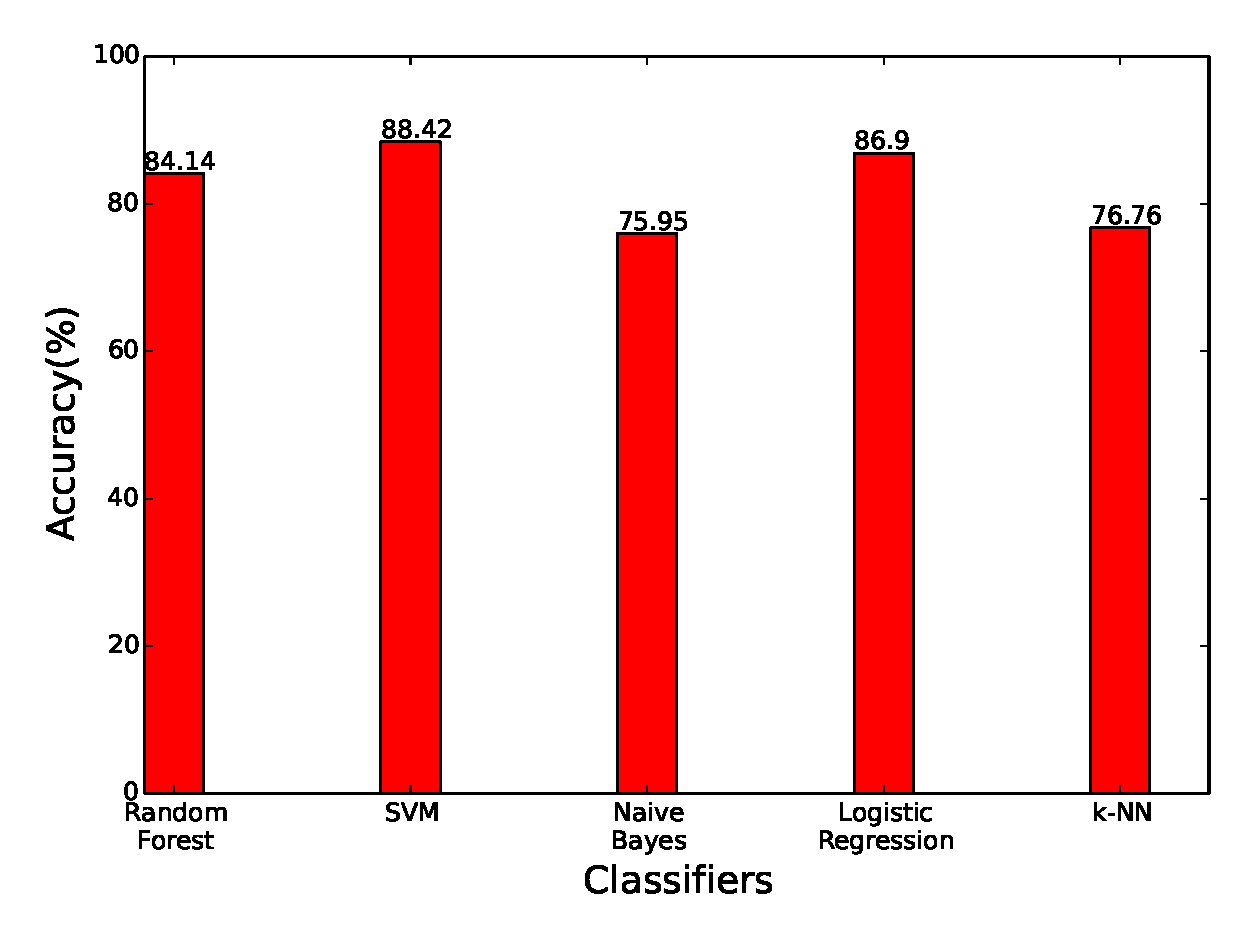
\includegraphics[width=140mm, height=120mm]{accuracy_wordvectors.eps}
\caption{Accuracies of Different Classifiers with Average Word Vectors(IMDB). \label{fig:accuracy_wordvectors}}
\end{figure}

\section{Results on Hindi Datasets}
\begin {table}[h!]
\centering
\begin{tabular}{ | c | c | c | }
\hline
\textbf{Features} & \textbf{Accuracy(1)} & \textbf{Accuracy(2)} \\ \hline
WordVector Averaging & 78.0 & 79.62\\ \hline
WordVector+tf-idf & 90.73 & 89.52\\ \hline
WordVector+tf-idf without stop words & \textbf{91.14} & \textbf{89.97}\\ \hline
\end{tabular}
\caption {Accuracies for Product Review and Movie Review Datasets.}
\end{table}

Table 3 represents the results using three different techniques for feature set construction. We see that there is a slight improvement in accuracy on both datasets once we remove stop-words.

\begin {table}[h!]
\centering
\begin{tabular}{ | c | c | c | }
\hline
\textbf{Experiment} & \textbf{Features} & \textbf{Accuracy} \\ \hline
Word Vector with SVM (Our method) & tf-idf with word vector & \textbf{91.14}\\ \hline
Subjective Lexicon (Bakliwal et al.(2012)) & Simple Scoring & 79.03\\ \hline
Hindi-SWN Baseline (Arora et al.(2013)) & Adjective and Adverb presence & 69.30\\ \hline
\end{tabular}
\caption {Comparison of Approaches: Product Review Dataset}
\end{table}
Table 4 and 5 compares our best method with various other methods which have performed well using techniques such as \emph{tf-idf}, subjective lexicon, etc.

\begin {table}[h!]
\centering
\begin{tabular}{ | c | c | c | }
\hline
\textbf{Experiment} & \textbf{Features} & \textbf{Accuracy} \\ \hline
WordVector Averaging & word vector & 78.0\\ \hline
Word Vector with SVM (Our method) & tf-idf; word vector & \textbf{89.97}\\ \hline
In language using SVM (Joshi et al.(2010)) & tf-idf & 78.14\\ \hline
MT Based using SVM (Joshi et al.(2010)) & tf-idf & 65.96\\ \hline
Improved Hindi-SWN  (Bakliwal et al.(2012)) & Adj. and Adv. presence & 79.0\\ \hline
\end{tabular}
\caption {Comparison of Approaches: Movie Review Dataset}
\end{table}

Table 5 shows the top few similar words for certain words from the corpus with cosine similarity as a distance metric. 
The words which have higher cosine similarity tend to be semantically and syntactically related.
\begin {table}[h!]
\small
\begin{tabular}{ | l | l | l | }
\hline
\textbf{{\dn aQCA}} & \textbf{{\dn{KrAb}}} & \textbf{{\dn ByAnk}} \\ \hline
{\dn b\7{h}t} & {\dn EnrAsAjnk} & {\dn By\306wkr}\\ \hline
{\dn \7{s}pr} & {\dn kM)or} & {\dn BFqZ}\\ \hline
{\dn k\?vl} & {\dn nA\7{)}k} & {\dn ByAvh}\\ \hline
{\dn itnA} & {\dn bdtr} & {\dn avsAd}\\ \hline
\end{tabular}
\caption {Some sentiment words and their neighbors}
\end{table}
